% supplementary.tex - Standalone supplementary information
%
% Compile with: pdflatex supplementary.tex (twice for cross-references)
%
\documentclass[12pt]{article}

\usepackage[letterpaper,margin=1.0in,top=1.0in,bottom=1.0in]{geometry}
\usepackage{setspace}
\usepackage{amsmath,amssymb}
\usepackage{booktabs}
\usepackage{graphicx}
\usepackage{xcolor}
\usepackage{hyperref}
\usepackage{microtype}
\usepackage{caption}
\usepackage{multirow}
\usepackage[numbers,super,sort&compress]{natbib}

\hypersetup{colorlinks=true,linkcolor=blue!60!black,citecolor=blue!60!black,urlcolor=blue!60!black}
\captionsetup{font=small,labelfont=bf,skip=4pt}

\renewcommand{\thetable}{S\arabic{table}}
\renewcommand{\thefigure}{S\arabic{figure}}

\title{\large\bfseries Supplementary Information for\\[4pt]
\normalsize Policy Recovery and No-Count Bet-Sizing Optimality in Infinite-Shoe Blackjack}

\begin{document}

\maketitle
\thispagestyle{plain}

\section*{Supplementary Information}

\subsection*{S1. Optimizer hyperparameters}

Table~\ref{tab:hparams} lists the hyperparameters used in all experiments.

\begin{table}[h]
\centering
\caption{Hyperparameters used in all experiments.}
\label{tab:hparams}
\small
\begin{tabular}{lll}
\toprule
Method & Parameter & Value \\
\midrule
\multirow{6}{*}{PG}
  & Learning rate $\eta$ & $3 \times 10^{-3}$ \\
  & Batch size $|B|$ & $64$ \\
  & Entropy coef.\ $\lambda_{H,0}$ & $0.05$ \\
  & Entropy anneal & $0.99995$ per hand \\
  & Baseline EMA $\alpha_b$ & $0.02$ \\
  & Adam $(\beta_1, \beta_2)$ & $(0.9,\,0.999)$ \\
\midrule
\multirow{6}{*}{SPSA}
  & $a$, $c$ & $0.5$, $0.2$ \\
  & $\alpha$, $\gamma$ & $0.602$, $0.101$ \\
  & $A$ & $100$ \\
  & $n_\mathrm{eval}$ per side & $300$ \\
  & Iterations & $8{,}000$ \\
\midrule
\multirow{6}{*}{CEM}
  & Population size $N$ & $50$ \\
  & Elite fraction $\rho$ & $0.20$ \\
  & $n_\mathrm{eval}$ per policy & $500$ \\
  & $\sigma_0$ & $2.0$ \\
  & $\sigma_\mathrm{min}$ & $0.05$ \\
  & Noise decay & $0.995$ per gen.\ \\
\bottomrule
\end{tabular}
\end{table}

\subsection*{S2. Rule variant sensitivity}

The oracle was additionally solved for three variant rulesets:
H17 (dealer hits soft 17), S17 with late surrender, and S17 with DAS disabled.
Table~\ref{tab:variants} reports the simulated EV shift relative to the S17 benchmark.

\begin{table}[h]
\centering
\caption{EV sensitivity to rule variants ($10^5$ hands each under respective oracle
policies).}
\label{tab:variants}
\small
\begin{tabular}{lcc}
\toprule
Ruleset & EV & $\Delta$ vs.\ S17 \\
\midrule
S17 (benchmark) & $-0.00476$ & N/A \\
H17             & $-0.00692$ & $-0.00216$ \\
S17 + Surrender & $-0.00398$ & $+0.00078$ \\
S17, no DAS     & $-0.00614$ & $-0.00138$ \\
\bottomrule
\end{tabular}
\end{table}

The H17 penalty ($-0.22\%$) and DAS removal ($-0.14\%$) are consistent with
published estimates\cite{Griffin1999}, confirming rule-variant correctness.  Late
surrender contributes $+0.08\%$, also within $0.01\%$ of published figures.

\clearpage
\subsection*{S3. Regret heatmaps for SPSA and CEM}

Figures~\ref{fig:spsa_hard}--\ref{fig:cem_pair} present the exported regret heatmaps
for SPSA and CEM on hard totals, soft totals, and pair cells.

\begin{figure}[p]
\centering
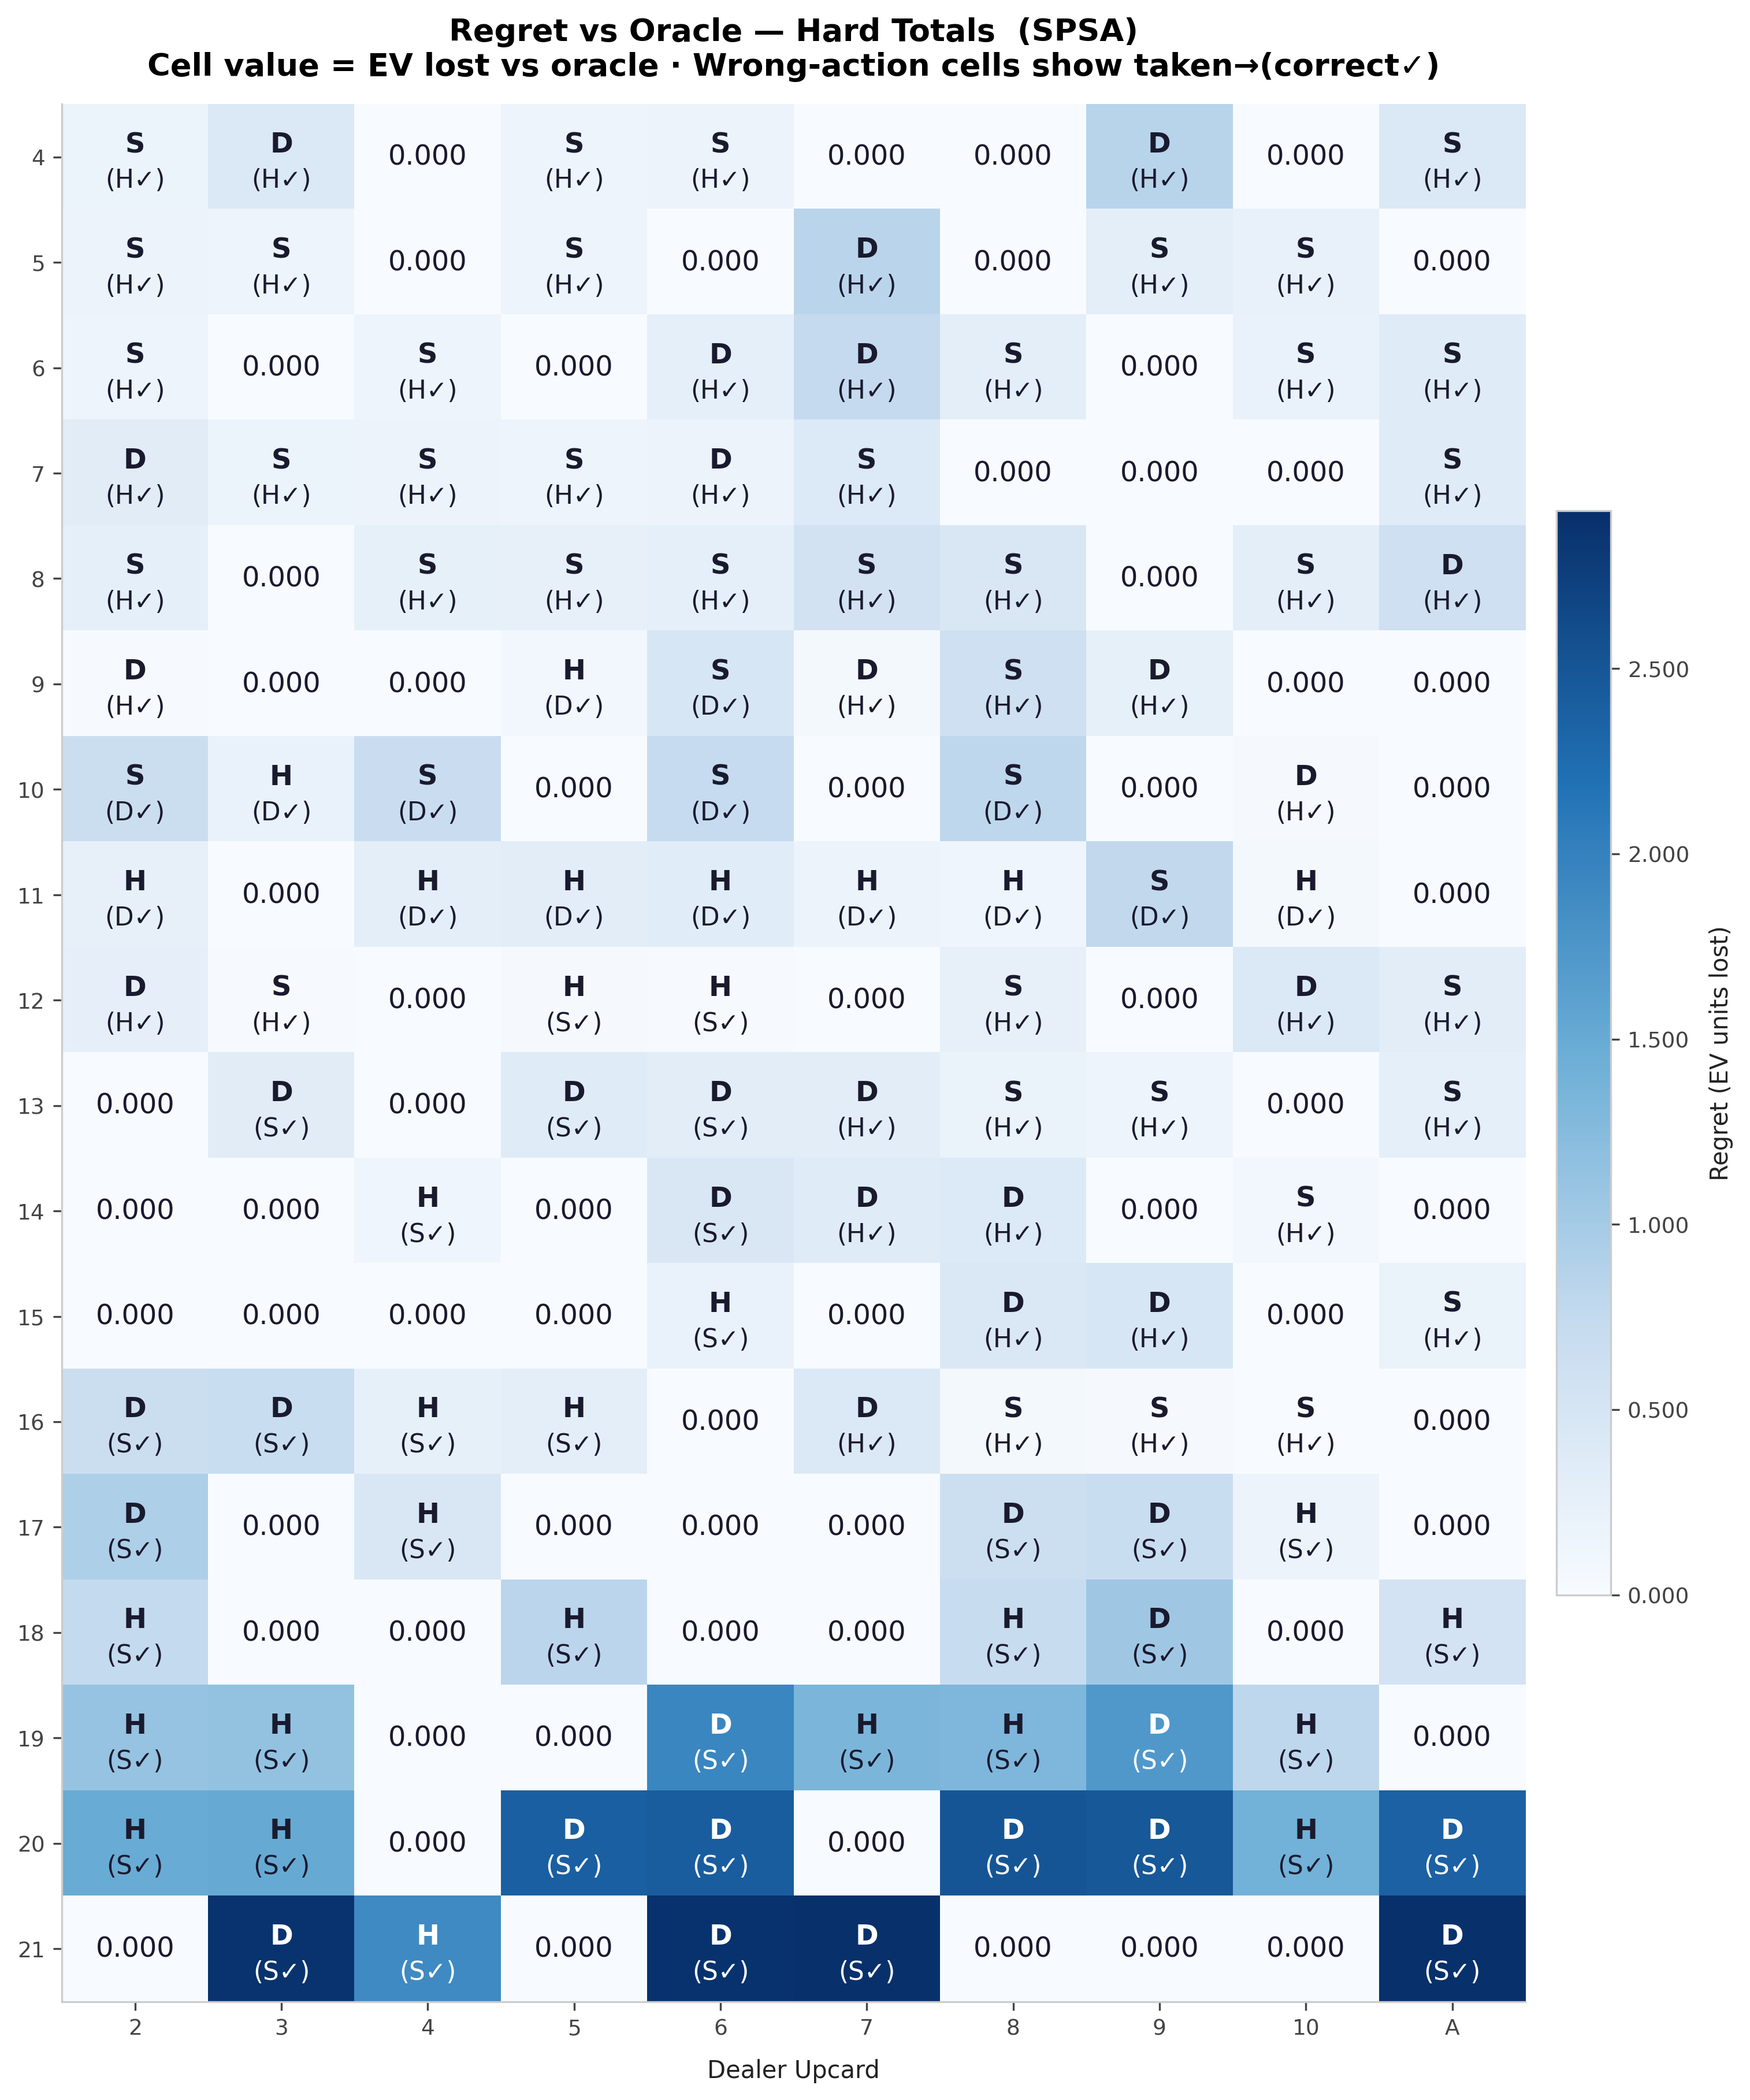
\includegraphics[width=0.95\textwidth]{figures/SPSA_regret_hard.png}
\caption{SPSA regret heatmap for hard totals.}
\label{fig:spsa_hard}
\end{figure}

\begin{figure}[p]
\centering
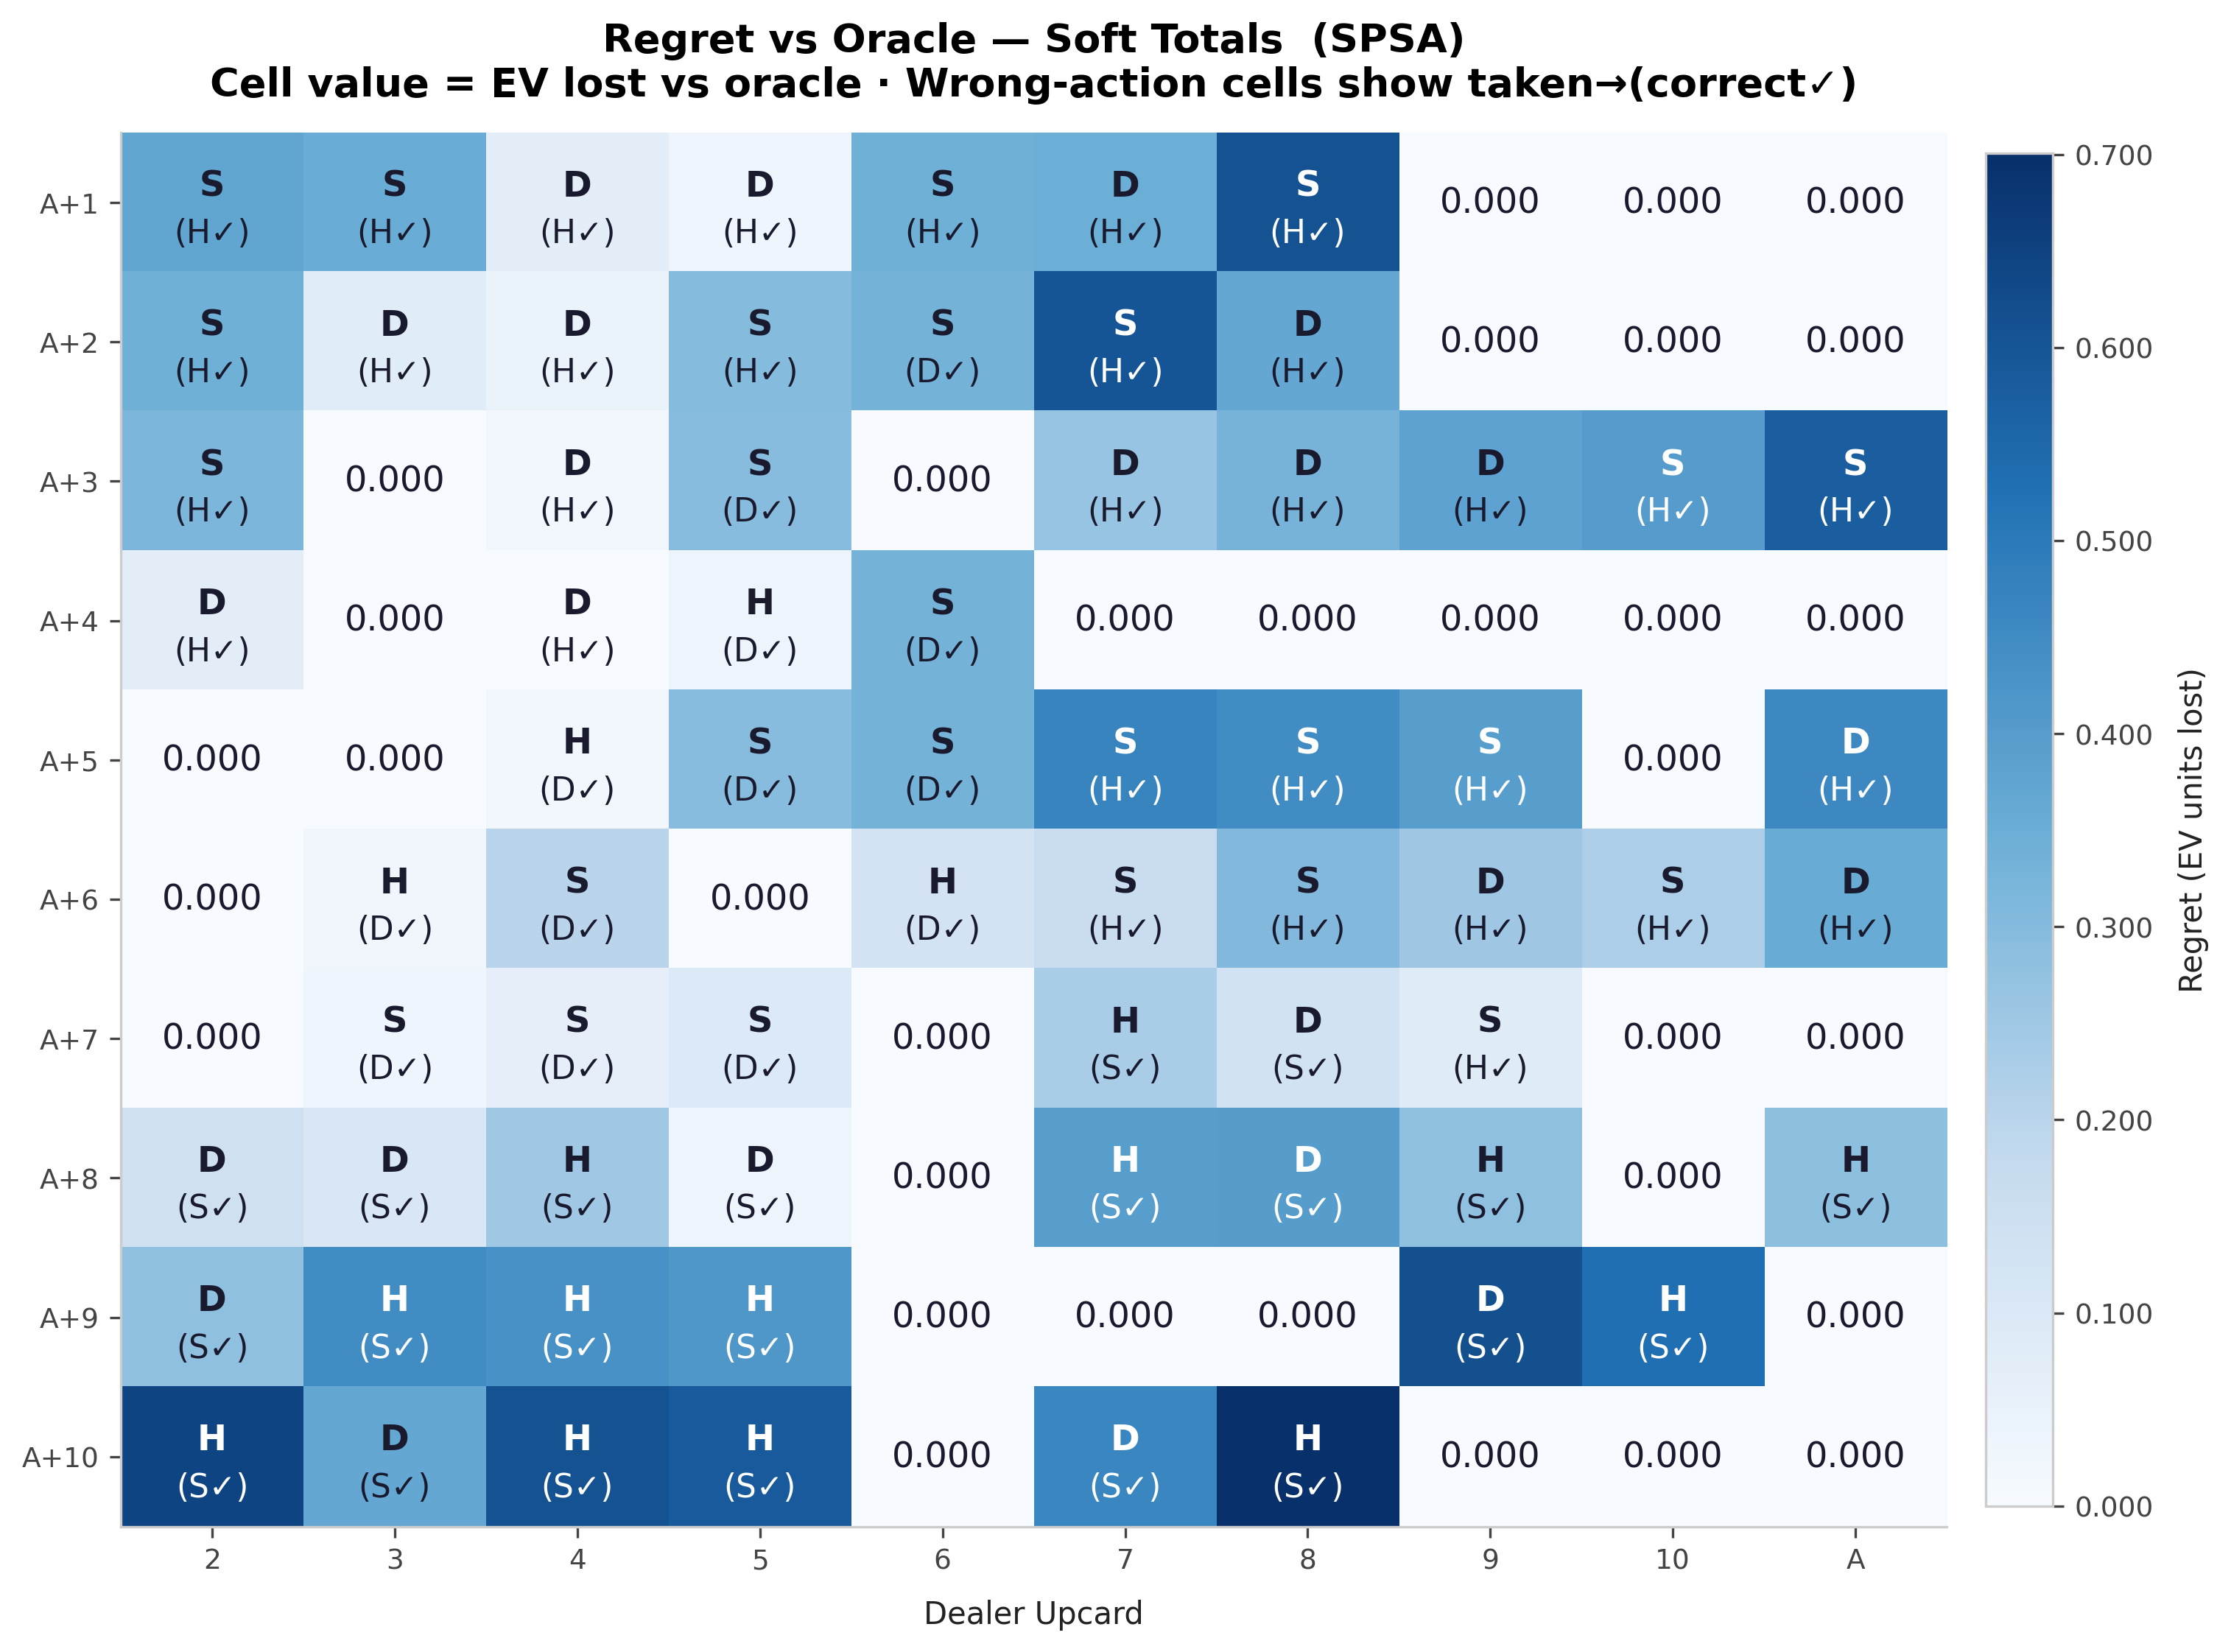
\includegraphics[width=0.95\textwidth]{figures/SPSA_regret_soft.png}
\caption{SPSA regret heatmap for soft totals.}
\label{fig:spsa_soft}
\end{figure}

\begin{figure}[p]
\centering
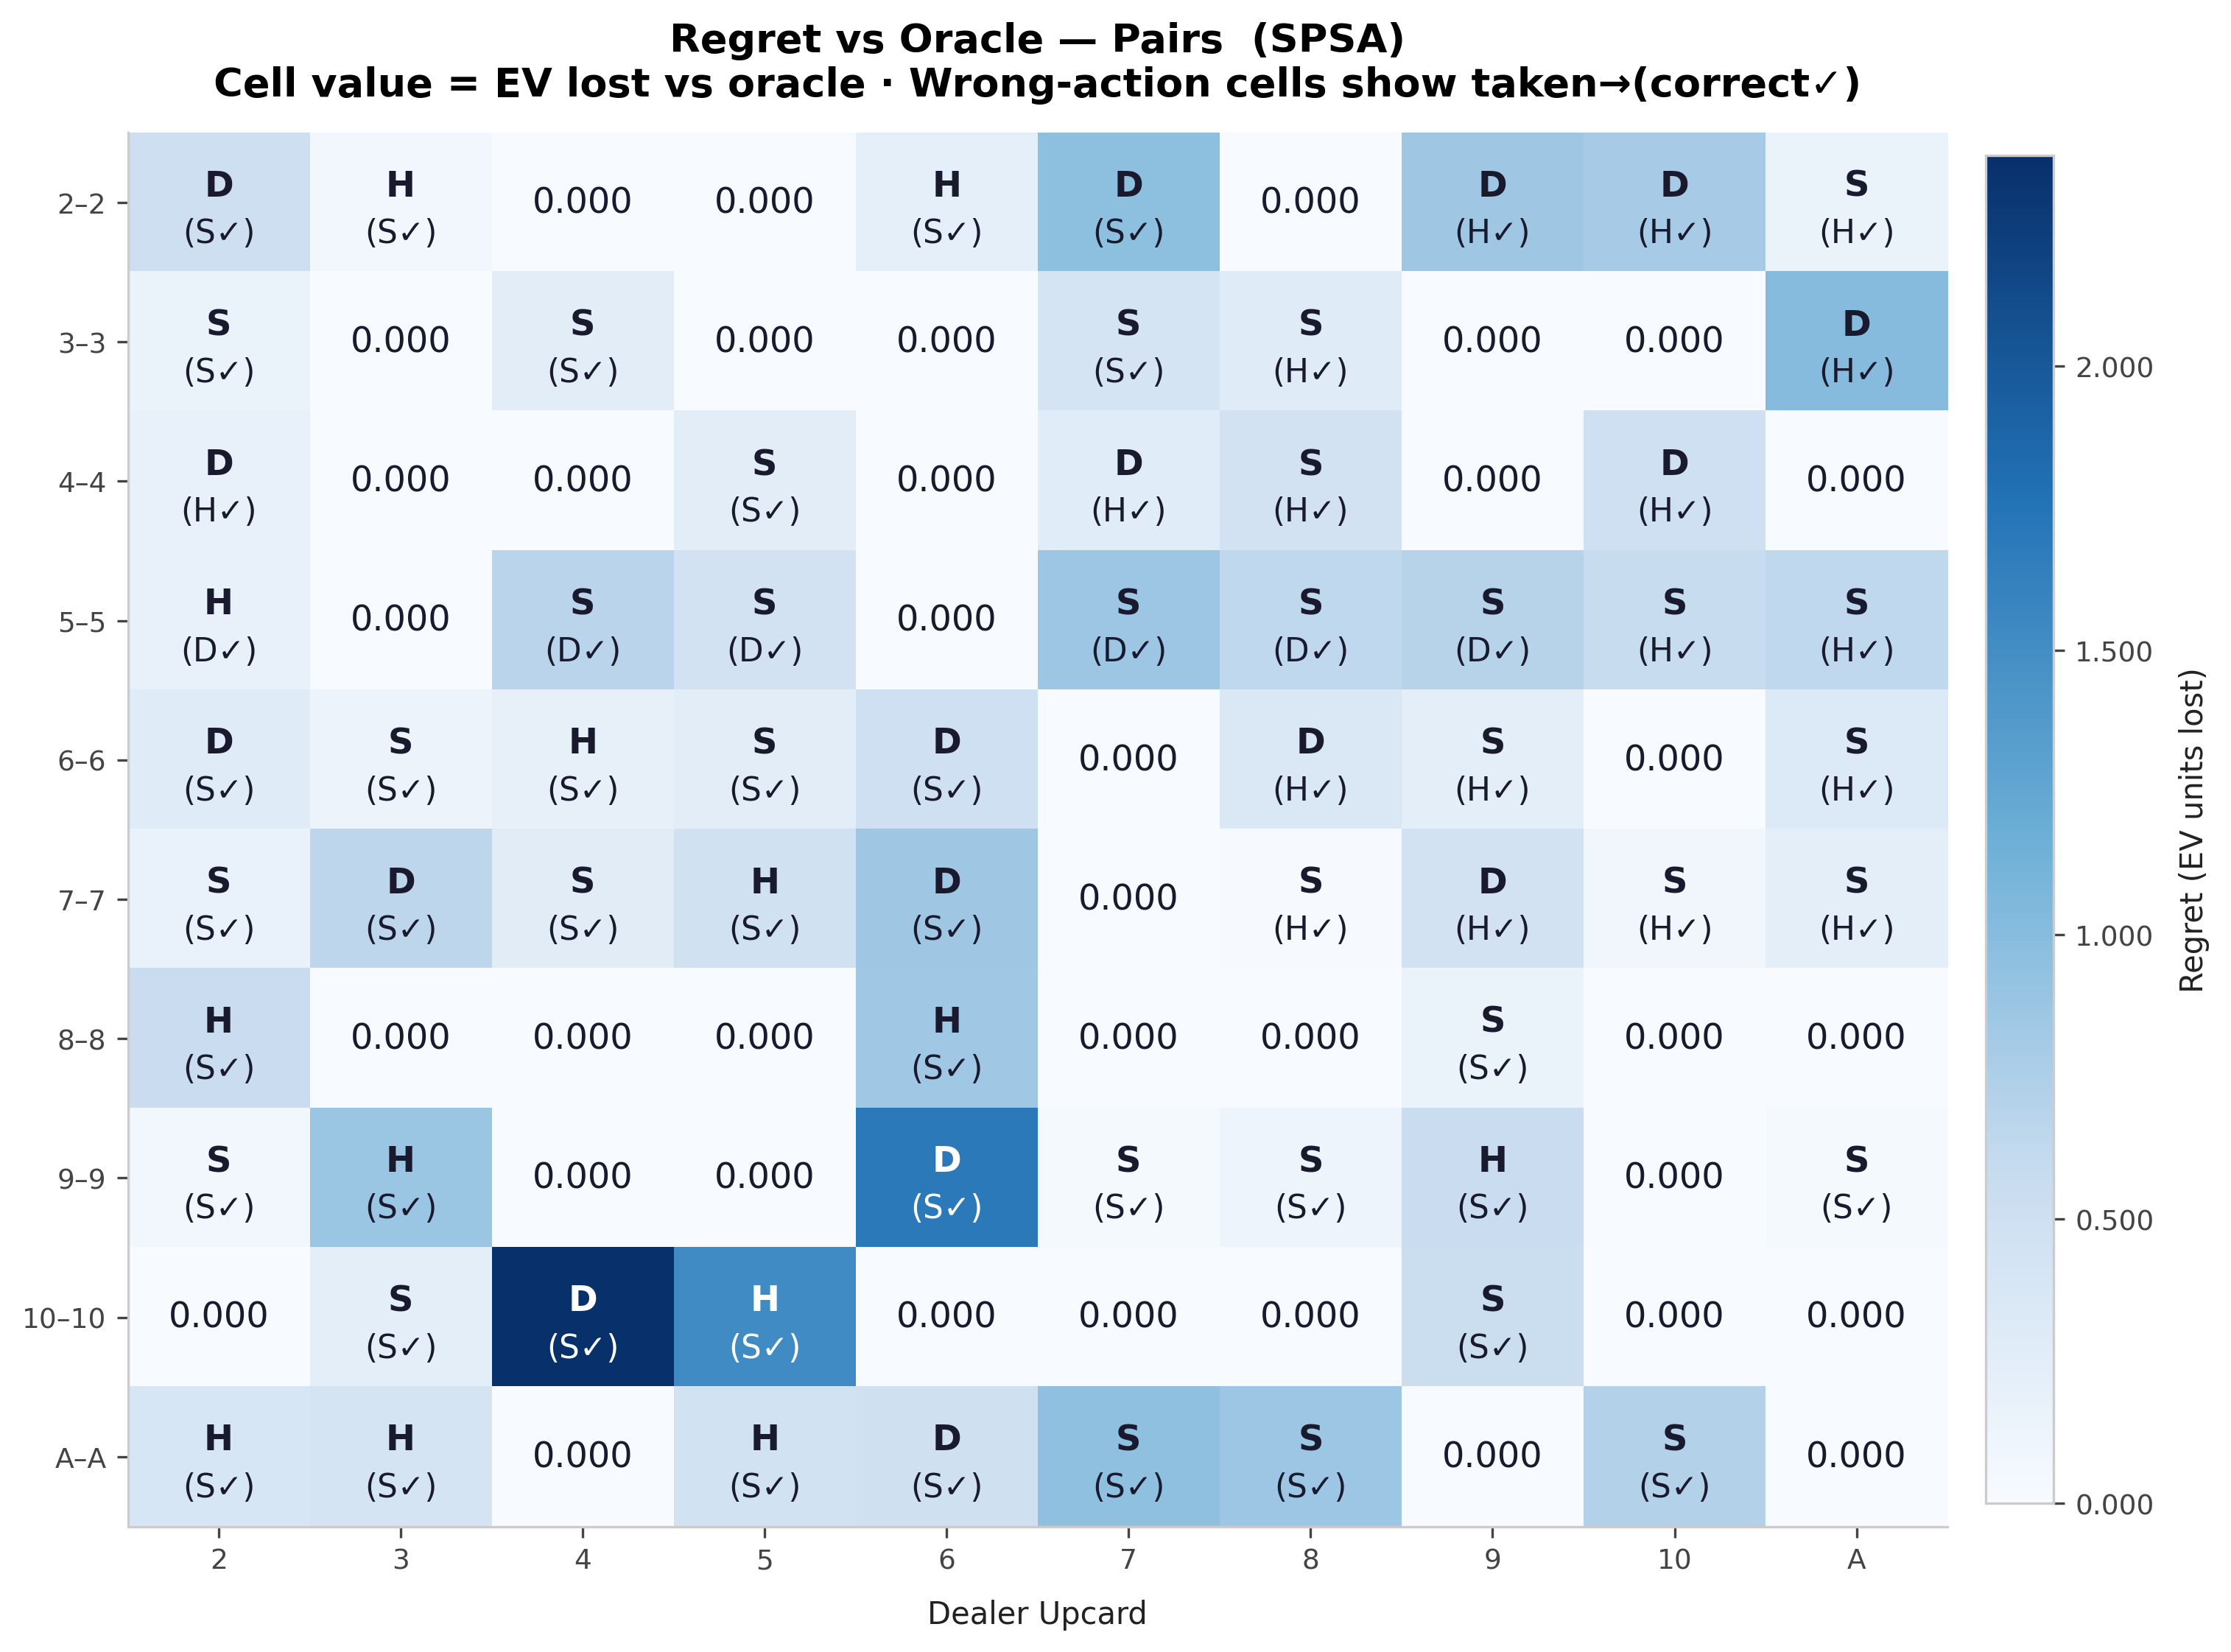
\includegraphics[width=0.95\textwidth]{figures/SPSA_regret_pair.png}
\caption{SPSA regret heatmap for pair cells.}
\label{fig:spsa_pair}
\end{figure}

\begin{figure}[p]
\centering
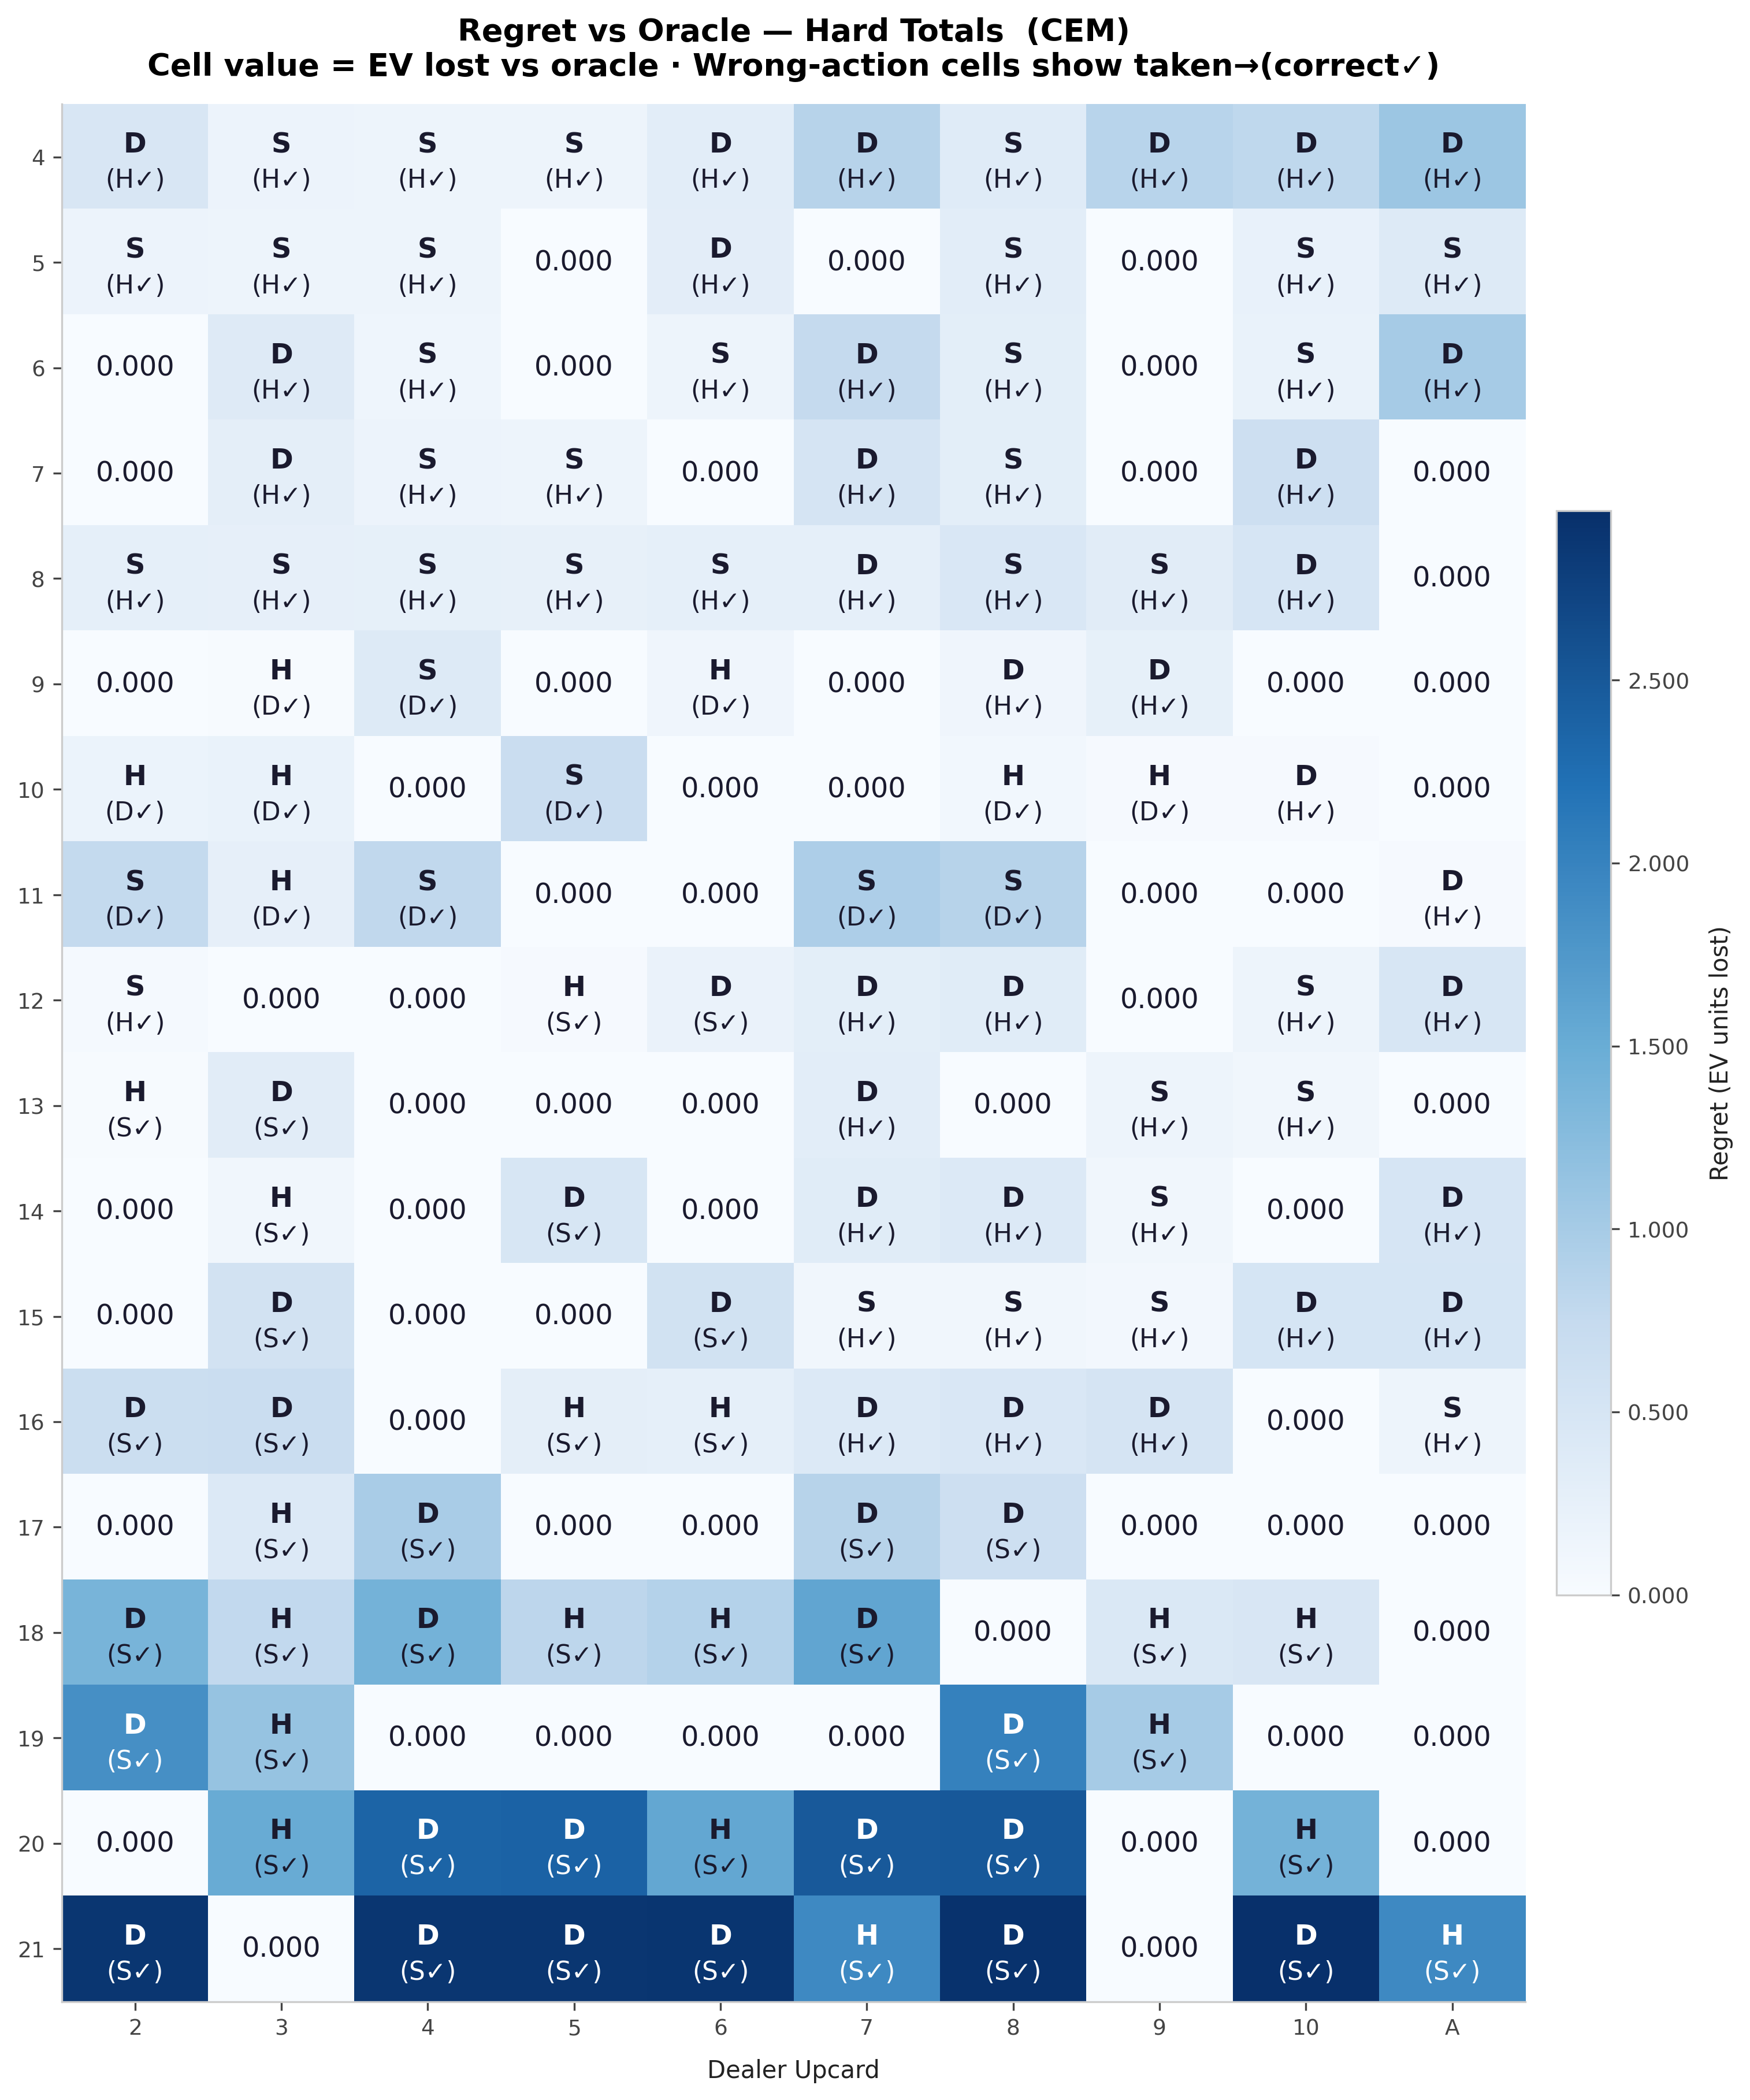
\includegraphics[width=0.95\textwidth]{figures/CEM_regret_hard.png}
\caption{CEM regret heatmap for hard totals.}
\label{fig:cem_hard}
\end{figure}

\begin{figure}[p]
\centering
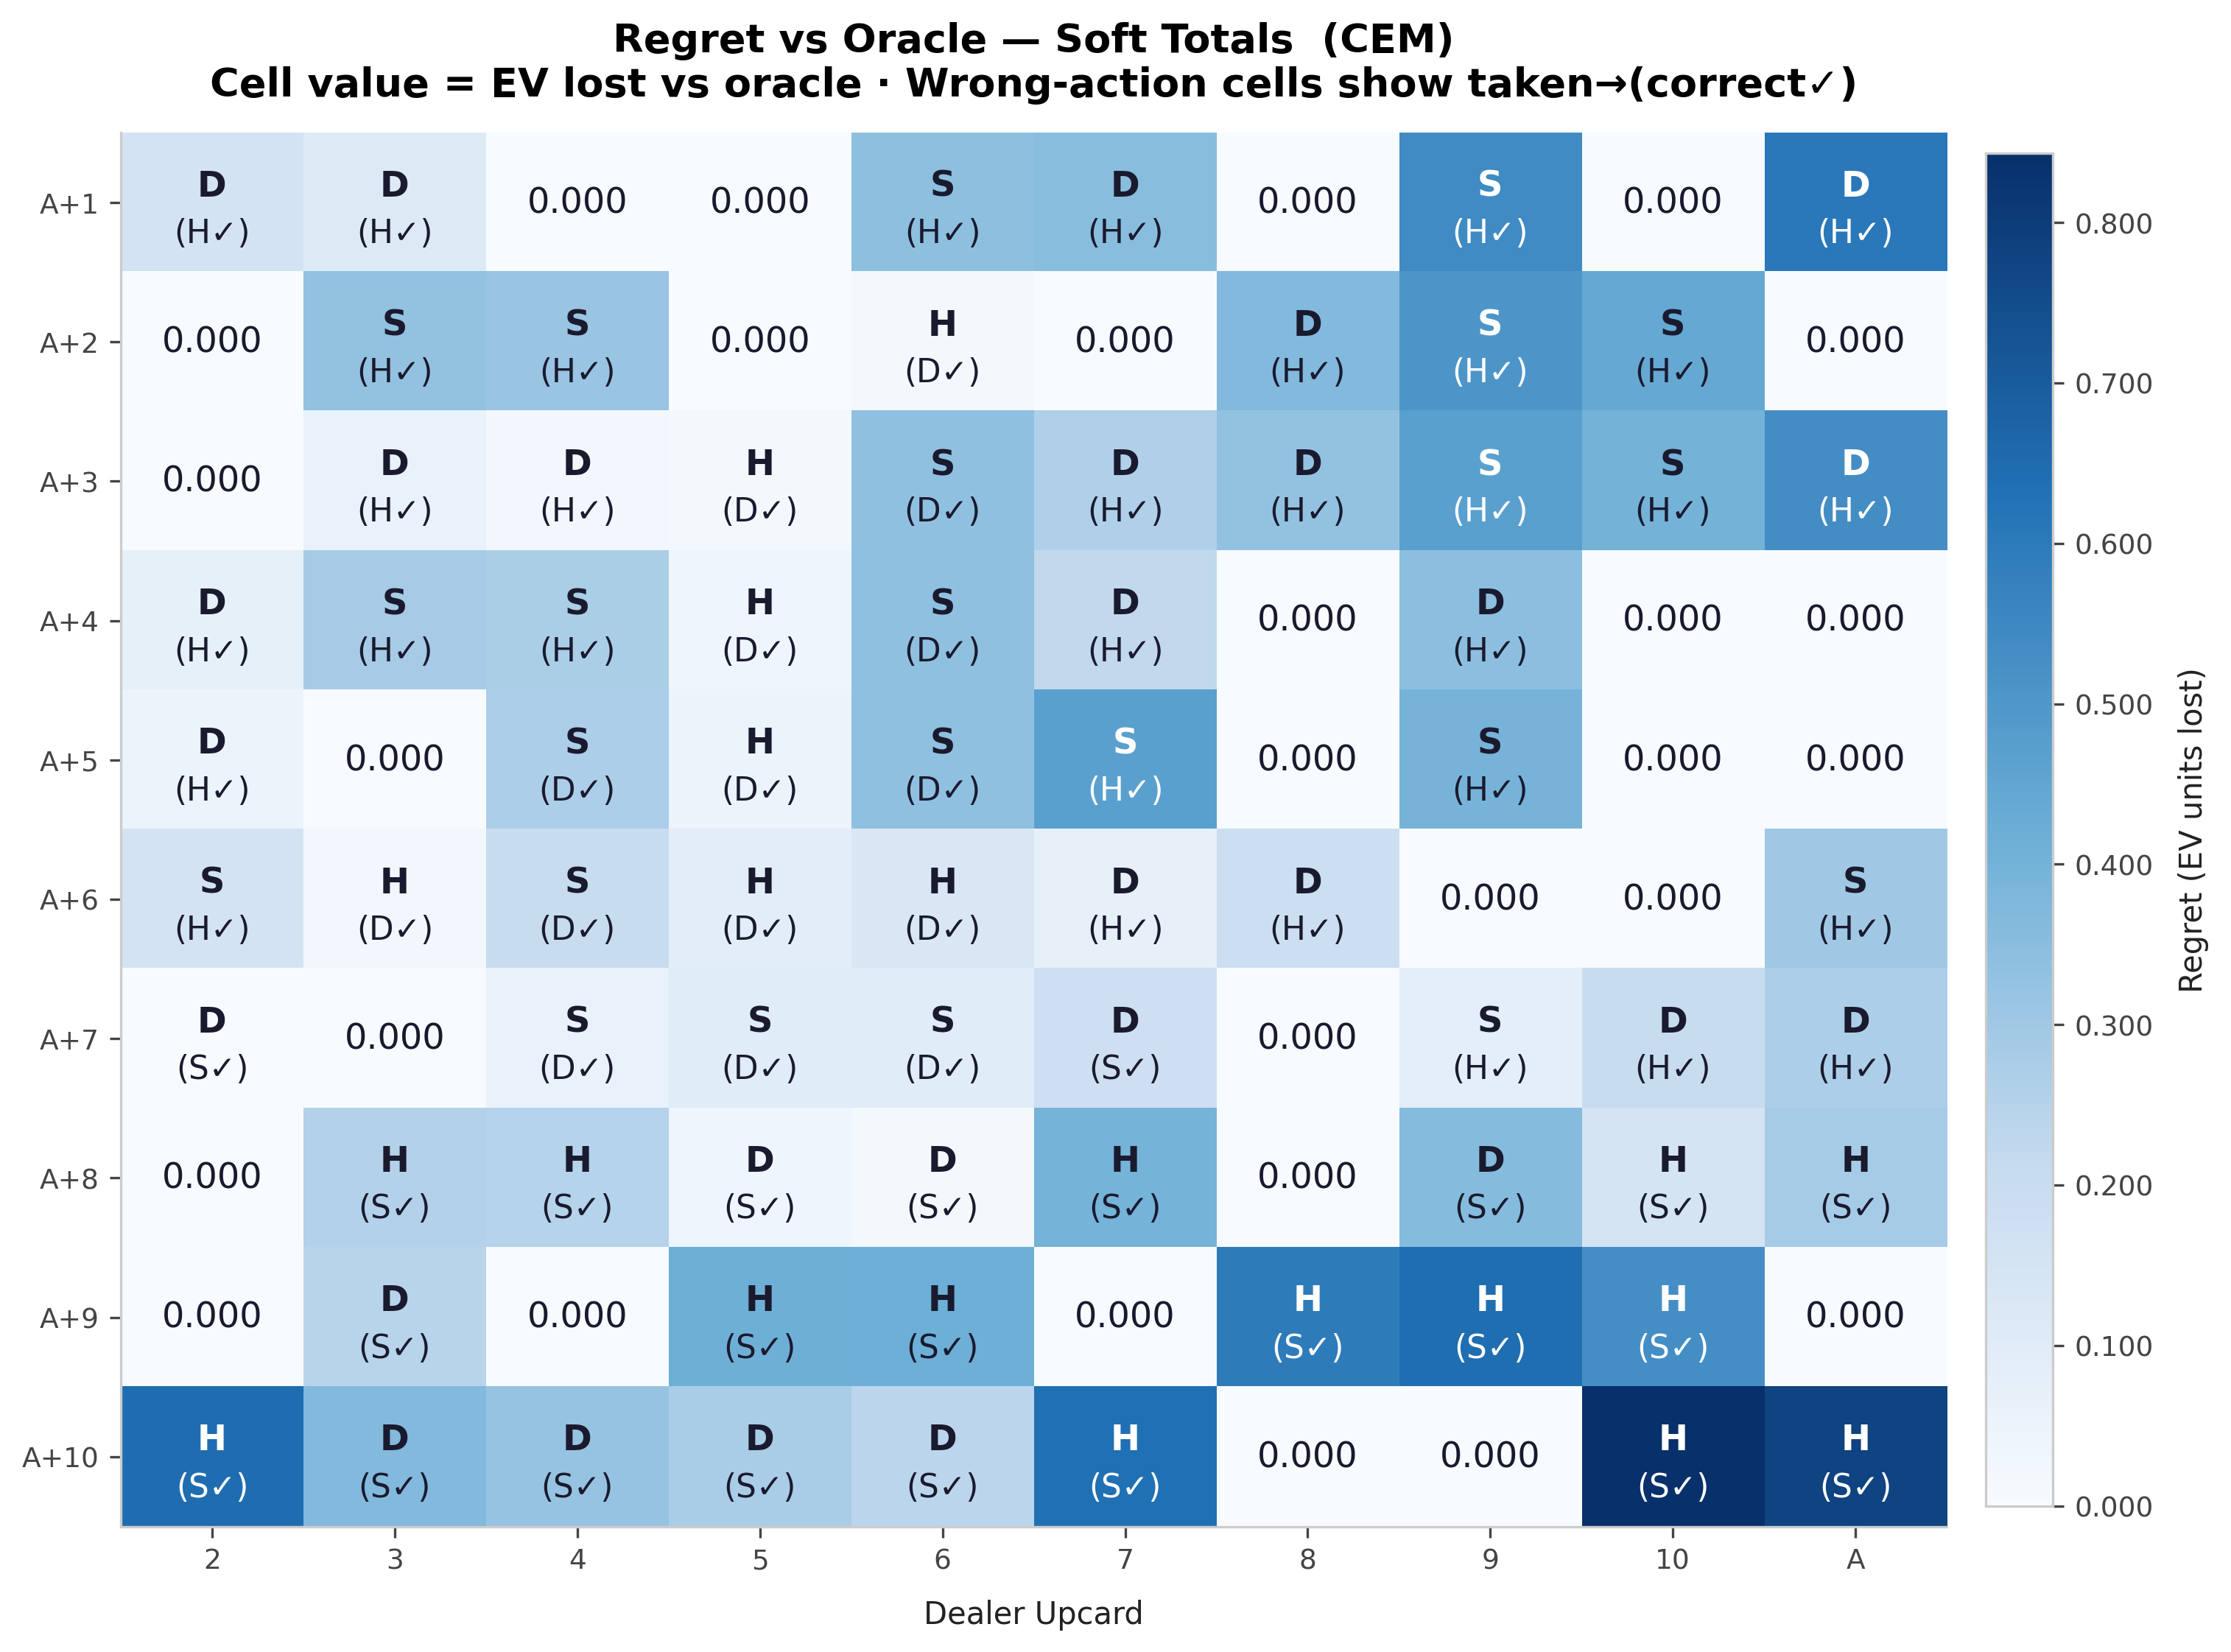
\includegraphics[width=0.95\textwidth]{figures/CEM_regret_soft.png}
\caption{CEM regret heatmap for soft totals.}
\label{fig:cem_soft}
\end{figure}

\begin{figure}[p]
\centering
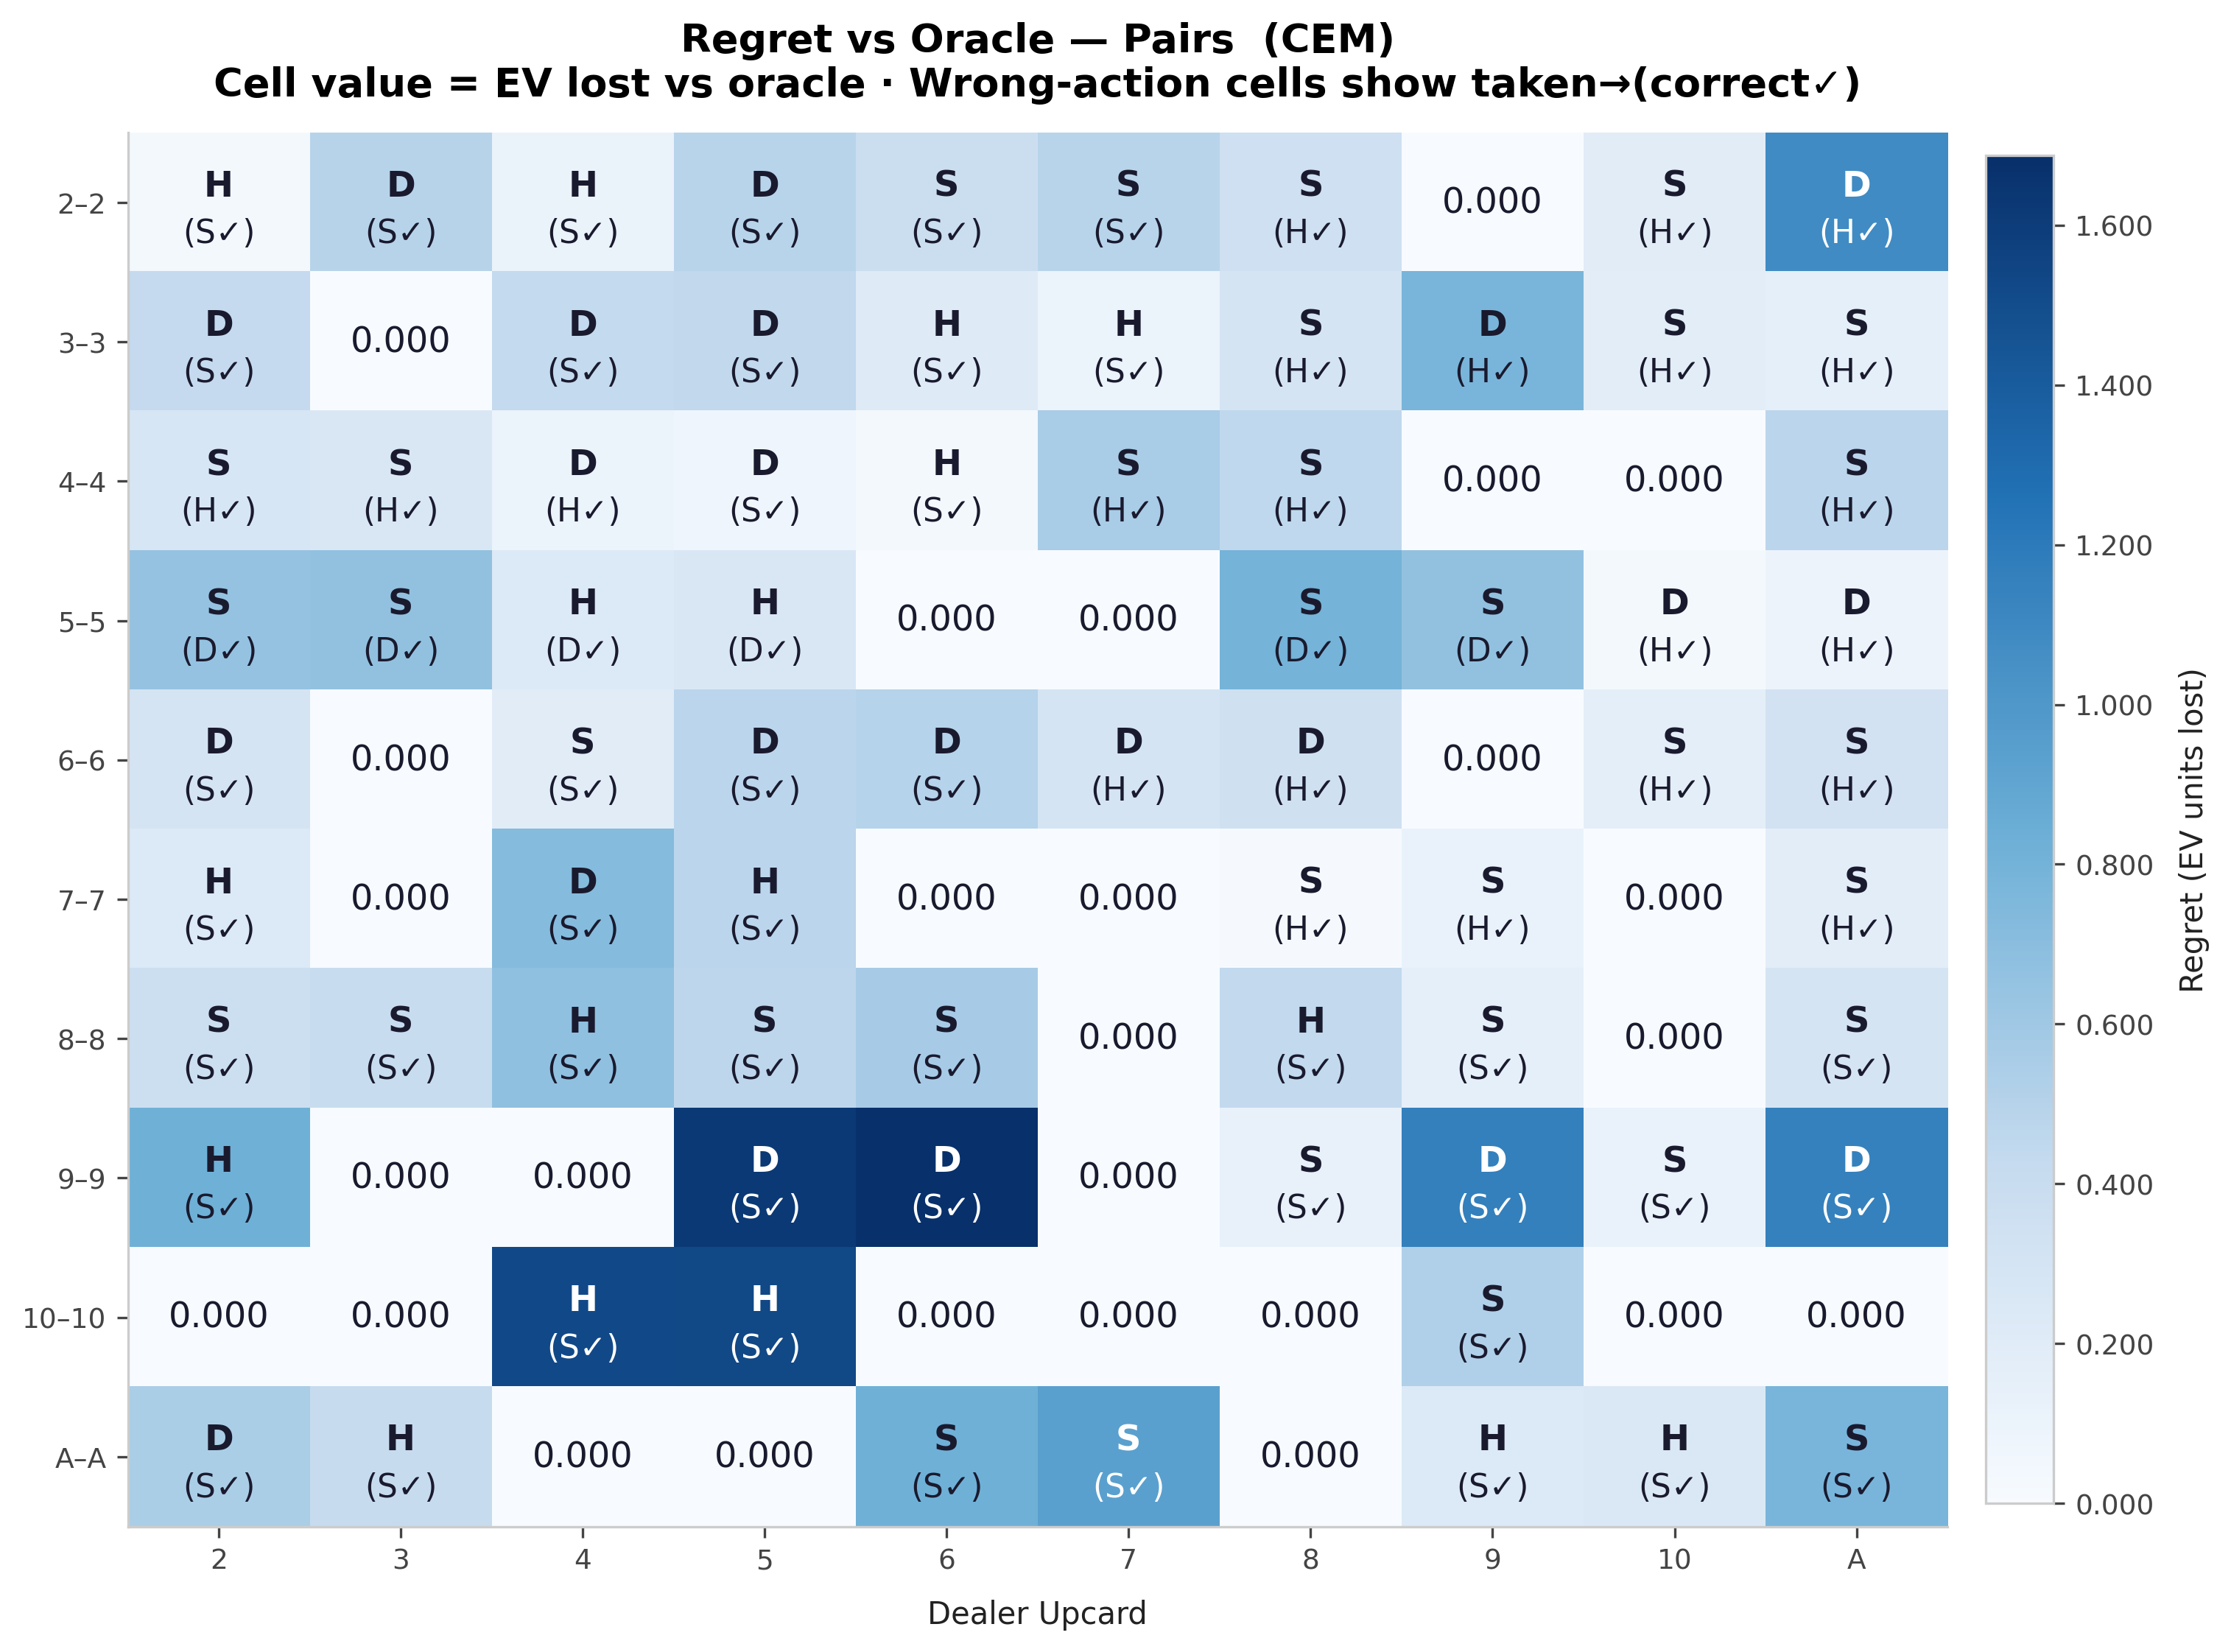
\includegraphics[width=0.95\textwidth]{figures/CEM_regret_pair.png}
\caption{CEM regret heatmap for pair cells.}
\label{fig:cem_pair}
\end{figure}

The hard-total regret maps show that SPSA leaves more residual error distributed
across the chart, while CEM concentrates errors on a narrower subset of cells at
higher magnitude.

\clearpage
\subsection*{S4. Proof of ruin probability monotonicity}

Let $W_n = W_0 + \sum_{t=1}^n b R_t$ be the bankroll random walk with constant bet
$b$ and i.i.d.\ $R_t$ with mean $e < 0$ and variance $\sigma^2 > 0$.  By the Wald
identity, $\mathbb{E}[W_\tau] = W_0 + b\,e\,\mathbb{E}[\tau]$ where $\tau$ is the
ruin time; the optional stopping theorem confirms that for the walk with absorbing
barrier at 0, $P(\tau < \infty) = 1$.  The ruin probability before $N$ fixed steps,
$P(\min_{1 \le t \le N} W_t \le 0)$, is monotone increasing in $b$ for fixed $W_0$,
because scaling $b \to \lambda b$ ($\lambda > 1$) is equivalent to scaling
$W_0 \to W_0/\lambda$, which strictly increases ruin probability under a
negative-drift random walk.  Therefore minimum bet minimizes ruin probability
for all $N$ and $W_0$.

\begin{thebibliography}{9}

\bibitem{Griffin1999}
Griffin, P.\ A.
\textit{The Theory of Blackjack: The Compleat Card Counter's Guide to the Casino Game
of 21}, 6th edn (Huntington Press, Las Vegas, 1999).

\end{thebibliography}

\end{document}
